% L10b student companion deck: a review of the Greeks, the POE, and the POP; then
% composite contracts, their net present value and profit at expiration, the common
% credit structures (short puts and calls, credit spreads, short straddles and
% strangles, protected strangles and iron condors), and why we wait to expiration.
%
% The frame order mirrors the lecture notebook. The disclaimer is slide 2, by
% instructor preference. Notation follows the lecture: composite contract
% \mathcal{C} with legs i, orientation \theta_i, copy number n_i, strike K_i, leg
% payoff V_i(K_i,S(T)), composite payoff \hat{V}_{\mathcal{C}}(S(T)), composite premium
% \mathcal{P}_{\mathcal{C}}, profit at expiration \hat{P}_{\mathcal{C}}(S(T)),
% discount factor \mathcal{D}^{-1}_{T,0}(g_y), accumulation factor
% \mathcal{D}_{T,0}(g_y) (always written in full), and breakevens S^{\ddagger},
% S^{\ddagger}_{\pm}. October 28, 2026: the POE/POP pseudocode frames from L10a
% added to the review (S_0 -> S(0), \mathcal{P} -> \Pc_{\star}, sample
% index i -> j because i is the leg index in L10b).
% Same day: the tastytrade company profile replaced by Akuna Capital.
% October 27, 2026: Delta hedging moved to L11a.
% October 26, 2026: first build, from the lecture after the October 26 scoring-round
% fixes. Figures are the light PDFs in ../figs (see ../figs/README.md).
% Same day, after the midterm feedback: a "What You Need to Know" frame (core results
% vs for understanding, mirroring the lecture's new box) follows the objectives, and
% every frame is tightened toward 60-80 words: closing sentences kept only when they
% state a result.
\documentclass[aspectratio=169,11pt]{beamer}
\usepackage{vnslides}

\newcommand{\Cc}{\mathcal{C}}
\newcommand{\Q}{\mathbb{Q}}
\newcommand{\Dc}{\mathcal{D}}
\newcommand{\Pc}{\mathcal{P}}
\newcommand{\repo}{https://github.com/varnerlab/CHEME-5660-CourseRepository-Fall-2026/blob/main/lectures/week-10/L10b}
\newcommand{\repoa}{https://github.com/varnerlab/CHEME-5660-CourseRepository-Fall-2026/blob/main/lectures/week-10/L10a}

\title{\texorpdfstring{{\vnheavy L10b}}{L10b}: The NPV and Probability of Profit of Composite Contracts}
\subtitle{CHEME 5660 Cornell University}
\author{Copyright Jeffrey Varner 2026. All Rights Reserved}

\begin{document}

\vntitlepage

\begin{frame}{Disclaimer and Risks}
  \vspace{0.6em}
  \textbf{\ink{Training only.}} This content is for training and informational
  purposes only. The teaching team does not make, give, or endorse any offer or
  solicitation to buy or sell securities or derivative products, or provide
  investment or trading advice or strategy.

  \vspace{1.1em}
  \textbf{\ink{Risk.}} Trading involves risk and is generally not recommended for
  those with limited resources, experience, or a low risk tolerance. Past
  performance does not guarantee future success.

  \vspace{1.1em}
  \textbf{\ink{Responsibility.}} You are responsible for your investment decisions
  based on your financial circumstances, objectives, risk tolerance, and
  liquidity needs.
\end{frame}

\begin{frame}{Objectives for Today}
  First, two examples on the Greeks, the POE, and the POP. Then: what is a
  composite contract worth, and when does it make money?

  \vspace{0.5em}
  {\large\textbf{\ink{Today's concepts}}}
  \begin{itemize}\setlength{\itemsep}{0.4em}
    \item \hilite{The POE and POP of a single contract}: from simulated share
      prices, compared with Delta.
    \item \hilite{The NPV and POP of a composite contract}: sums over its legs.
    \item \hilite{Common composite contracts}: outlook, breakevens, maximum profit
      and loss, and why closing early earns less.
  \end{itemize}
\end{frame}

\begin{frame}{What You Need to Know}
  \vspace{0.3em}
  {\large\textbf{\ink{Core concepts}}}
  \begin{itemize}\setlength{\itemsep}{0.4em}
    \item POE: the probability a contract finishes in the money. POP: the
      probability its profit at expiration is positive. Both come from simulated
      share prices, and the POE $\sim|\Delta_{\star}|$.
    \item Profit at expiration: the legs' payoffs, weighted by $\theta_{i}n_{i}$,
      minus the composite premium grown to expiration. POP: the probability it is
      positive.
    \item Read a profit diagram: the breakevens, the maximum profit (the credit
      grown to expiration), and the maximum loss. Closing early earns less, by
      roughly the extrinsic value left in the legs.
  \end{itemize}

  \vspace{0.5em}
  {\large\textbf{\ink{For understanding}} \dimmed{(you won't reproduce these)}}
  \begin{itemize}\setlength{\itemsep}{0.3em}
    \item The NPV derivation and the formula tables for the eight composite
      contracts.
  \end{itemize}
\end{frame}

\begin{frame}{Lectures and Examples}
  \vspace{0.3em}
  {\normalsize\textbf{\ink{Lecture:}}\par\small
  \href{\repo/CHEME-5660-L10b-Lecture-POP-POE-Delta-CompositeContracts-Fall-2026.ipynb}{\dimmed{CHEME-5660-L10b-Lecture-POP-POE-Delta-CompositeContracts-Fall-2026.ipynb}}}

  \vspace{0.6em}
  {\normalsize\textbf{\ink{Example 1:}}\par\small
  \href{\repoa/CHEME-5660-L10a-Example-Greeks-PutCall-Fall-2026.ipynb}{\dimmed{CHEME-5660-L10a-Example-Greeks-PutCall-Fall-2026.ipynb}}}

  \vspace{0.45em}
  {\normalsize\textbf{\ink{Example 2:}}\par\small
  \href{\repoa/CHEME-5660-L10a-Example-POE-POP-Call-Fall-2026.ipynb}{\dimmed{CHEME-5660-L10a-Example-POE-POP-Call-Fall-2026.ipynb}}}

  \vspace{0.45em}
  {\normalsize\textbf{\ink{Example 3:}}\par\small
  \href{\repo/CHEME-5660-L10b-Example-Delta-VerticalSpread-Fall-2026.ipynb}{\dimmed{CHEME-5660-L10b-Example-Delta-VerticalSpread-Fall-2026.ipynb}}}

  \vspace{0.45em}
  {\normalsize\textbf{\ink{Review on your own:}}\par\small
  \href{\repo/CHEME-5660-L10b-Example-Straddle-AMD-Earnings-Fall-2026.ipynb}{\dimmed{CHEME-5660-L10b-Example-Straddle-AMD-Earnings-Fall-2026.ipynb}}}
\end{frame}

% ========== Review: The Greeks, POE, and POP
\begin{frame}{Review: The Greeks}
  For small changes in the share price, the volatility, the calendar time
  (years), and the rate, the premium $\Pc_{\star}$ of a call ($\star=c$) or put
  ($\star=p$) changes by:
  \begin{align*}
    \Delta\Pc_{\star}&\approx\Delta_{\star}\,\Delta S+\tfrac{1}{2}\,\Gamma_{\star}\,(\Delta S)^{2}
    +\nu_{\star}\,\Delta\sigma+\Theta_{\star}\,\Delta t+\rho_{\star}\,\Delta g_{y}\\
    &=\underbrace{\bigl(\Delta_{\star}+\tfrac{1}{2}\,\Gamma_{\star}\,\Delta S\bigr)\Delta S}_{\textstyle\text{share price}}
    +\underbrace{\nu_{\star}\,\Delta\sigma}_{\textstyle\text{volatility}}
    +\underbrace{\Theta_{\star}\,\Delta t}_{\textstyle\text{time}}
    +\underbrace{\rho_{\star}\,\Delta g_{y}}_{\textstyle\text{rate}}
  \end{align*}
  \begin{itemize}\setlength{\itemsep}{0.4em}
    \item \hilite{Delta and Gamma}: the slope and curvature of the premium in $S$.
    \item \hilite{Vega, Theta, and Rho}: sensitivities to the volatility $\sigma$,
      the calendar time $t$, and the risk-free rate $g_{y}$, quoted as
      $\Theta_{\star}/365$ per day and $\nu_{\star}/100$, $\rho_{\star}/100$ per point.
    \item \hilite{Hedge ratio}: one contract covers 100 shares, so it is
      equivalent to $100\cdot\Delta_{\star}$ shares.
  \end{itemize}
  \slidenote{Example 1:}{\href{\repoa/CHEME-5660-L10a-Example-Greeks-PutCall-Fall-2026.ipynb}{\dimmed{CHEME-5660-L10a-Example-Greeks-PutCall-Fall-2026.ipynb}}}
\end{frame}

\begin{frame}{Review: POE and POP}
  \vspace{0.3em}
  The \hilite{POE} is the probability of finishing in the money by more than 0.01~USD/share;
  the \hilite{POP} is the probability of a positive profit at expiration, beyond
  the breakeven $S^{\ddagger}=K\pm\Dc_{T,0}(g_{y})\cdot\Pc_{\star}$ ($+$ call, $-$ put):
  \begin{equation*}
    \boxed{
    \begin{aligned}
      \text{POE} &= \begin{cases}
      \mathbb{P}\left(S(T)>K+0.01\right) & \text{call}\\
      \mathbb{P}\left(S(T)<K-0.01\right) & \text{put}
      \end{cases}\\[0.3em]
      \text{POP} &= \begin{cases}
      \mathbb{P}\left(S(T)>S^{\ddagger}\right) & \text{bought a call or sold a put}\\
      \mathbb{P}\left(S(T)<S^{\ddagger}\right) & \text{sold a call or bought a put}
      \end{cases}
    \end{aligned}}
  \end{equation*}
  where $\Dc_{T,0}(g_{y})=e^{g_{y}T}$; we simulate $S(T)$ under our belief $\mathbb{P}$.
  However, the~POE~$\sim|\Delta_{\star}|$, the Delta quoted by trading platforms under $\Q$.
\end{frame}

\begin{frame}{Review: Computing POE and POP by Simulation}
  \vspace{0.3em}
  \hilite{Initialize}: given $S(0)$, $K$, the premium $\Pc_{\star}$ of the
  call or put, $T$ (years), the drift $\mu$ and volatility $\sigma$ under
  $\mathbb{P}$, $g_{y}$, and the number of samples $M$. Compute the breakeven
  $S^{\ddagger}$.
  \begin{enumerate}\setlength{\itemsep}{0.35em}
    \item For each sample $j=1,2,\dots,M$ \textbf{do}:
      \begin{itemize}
        \item[a.] Draw $Z_{j}\sim\mathcal{N}(0,1)$.
        \item[b.] Compute
          $S_{j}(T)\gets S(0)\exp\left[\left(\mu-\sigma^{2}/2\right)T+\sigma\sqrt{T}\,Z_{j}\right]$.
      \end{itemize}
    \item Compute the fraction of samples at or below each share price $x$:
      $\hat{F}(x)\gets\frac{1}{M}\cdot\#\left\{j:S_{j}(T)\leq x\right\}$.
  \end{enumerate}
\end{frame}

\begin{frame}{Review: Pseudocode for POE and POP}
  \vspace{0.3em}
  \begin{enumerate}\setlength{\itemsep}{0.45em}
    \setcounter{enumi}{2}
    \item If the contract is a call, \textbf{then}
      $\text{POE}\gets1-\hat{F}(K+0.01)$. Otherwise,
      $\text{POE}\gets\hat{F}(K-0.01)$.
    \item Compute the probability of profit:
      \begin{itemize}\setlength{\itemsep}{0.25em}
        \item If we bought a call or sold a put, \textbf{then}
          $\text{POP}\gets1-\hat{F}(S^{\ddagger})$.
        \item If we sold a call or bought a put, \textbf{then}
          $\text{POP}\gets\hat{F}(S^{\ddagger})$.
      \end{itemize}
  \end{enumerate}

  \vspace{0.6em}
  With $\mu=g_{y}$ and $\sigma$ set to the implied volatility, the same steps
  give the probabilities under $\Q$. These are the probabilities inside the
  market price, not our forecast.
  \slidenote{Example 2:}{\href{\repoa/CHEME-5660-L10a-Example-POE-POP-Call-Fall-2026.ipynb}{\dimmed{CHEME-5660-L10a-Example-POE-POP-Call-Fall-2026.ipynb}}}
\end{frame}

% ========== Company Profile: Akuna Capital
\begin{frame}{Company Profile: Akuna Capital}
  \href{https://akunacapital.com/what-we-do}{\hilite{Akuna Capital}}: an options
  market maker, headquartered in Chicago since 2011.
  \begin{itemize}\setlength{\itemsep}{0.4em}
    \item \hilite{Options market making}: it posts prices to buy and sell, trading
      with its own money (a proprietary trading firm).
    \item \hilite{Its own models}: it designs its own trading systems and models.
    \item \hilite{Teaching options}: a free
      \href{https://akunacapital.com/work-with-us/options-101/}{Options 101} course
      on payoff diagrams and the Greeks.
  \end{itemize}
  \vspace{0.3em}
  \textbf{\ink{Connection:}} a market maker may take the other side of one or
  both legs of the spread we sell. The quoted Delta comes from its premiums, so $|\Delta_{\star}|$ approximates each leg's
  POE under $\Q$, not under our forecast $\mathbb{P}$.
\end{frame}

% ========== Composite Contracts
\begin{frame}{Composite Contracts}
  A composite contract $\Cc$ combines long and short puts and calls on one
  underlying asset with one expiration date $T$. Its payoff per share at
  expiration is:
  \begin{equation*}
    \hat{V}_{\Cc}(S(T)) = \underbrace{\sum_{i\in\Cc}\theta_{i}\;n_{i}\;\overbrace{V_{i}(K_{i},S(T))}^{\textstyle\text{payoff of leg } i}}_{\textstyle\text{sum of all legs}}
  \end{equation*}
  Here $S(T)$ is the share price at expiration, $K_{i}$ the strike price of leg
  $i$, $V_{i}$ its payoff, $(S(T)-K_{i})^{+}$ for a call or $(K_{i}-S(T))^{+}$ for
  a put, $n_{i}$ its number of contracts, and $\theta_{i}=-1$ if short or $1$ if
  long.
\end{frame}

\begin{frame}{The Net Present Value of a Composite Contract}
  A composite contract is a sum of legs, so its NPV is the sum of the legs'
  NPVs, weighted by $\theta_{i}n_{i}$:
  \begin{align*}
    \operatorname{NPV}_{0}(\Cc) &= \sum_{i\in\Cc}\theta_{i}\,n_{i}\underbrace{\Bigl(-\Pc_{i}+\overbrace{\Dc^{-1}_{T,0}(g_{y})\cdot V_{i}(K_{i},S(T))}^{\textstyle\text{discounted payoff}}\Bigr)}_{\textstyle\text{NPV of buying leg } i} && \text{weighted leg NPVs}\\
    &= -\underbrace{\sum_{i\in\Cc}\theta_{i}\,n_{i}\,\Pc_{i}}_{\textstyle=\,\Pc_{\Cc}}+\Dc^{-1}_{T,0}(g_{y})\cdot\underbrace{\sum_{i\in\Cc}\theta_{i}\,n_{i}\,V_{i}(K_{i},S(T))}_{\textstyle=\,\hat{V}_{\Cc}(S(T))} && \text{split the sum}\\
    &= -\Pc_{\Cc}+\Dc^{-1}_{T,0}(g_{y})\cdot\hat{V}_{\Cc}(S(T))
  \end{align*}
  where $\Pc_{i}$ is the premium of leg $i$ (USD/share), positive whether we buy
  or sell it ($\theta_{i}$ sets the direction), and $\Pc_{\Cc}$ is the
  \hilite{composite premium}.
\end{frame}

\begin{frame}{Profit at Expiration}
  Factoring out $\Dc^{-1}_{T,0}(g_{y})$ writes the NPV as a profit at expiration
  discounted to today:
  \begin{align*}
    \operatorname{NPV}_{0}(\Cc) &= \Dc^{-1}_{T,0}(g_{y})\cdot\underbrace{\Bigl(\hat{V}_{\Cc}(S(T))-\Dc_{T,0}(g_{y})\cdot\Pc_{\Cc}\Bigr)}_{\textstyle=\,\hat{P}_{\Cc}(S(T))} && \text{factor out }\Dc^{-1}_{T,0}(g_{y})\\
    &= \Dc^{-1}_{T,0}(g_{y})\cdot\underbrace{\hat{P}_{\Cc}(S(T))}_{\makebox[0pt]{profit at expiration}}
  \end{align*}
  where $\Dc_{T,0}(g_{y})=e^{g_{y}T}$ is the accumulation factor, and:
  \begin{equation*}
    \boxed{\hat{P}_{\Cc}(S(T)) = \hat{V}_{\Cc}(S(T)) - \Dc_{T,0}(g_{y})\cdot\Pc_{\Cc}}
  \end{equation*}
  is the \hilite{profit at expiration} (USD/share). $\Pc_{\Cc}>0$ opens for a
  \hilite{debit}; $\Pc_{\Cc}<0$ opens for a \hilite{credit} of $-\Pc_{\Cc}$.
\end{frame}

\begin{frame}{Probability of Profit and Probability of Exercise}
  The NPV and the profit at expiration have the same sign, so with $\mathbb{P}$
  our belief, the \hilite{probability of profit} is:
  \begin{equation*}
    \boxed{\text{POP}_{\Cc} = \mathbb{P}\Bigl(\operatorname{NPV}_{0}(\Cc)>0\Bigr) = \mathbb{P}\Bigl(\hat{P}_{\Cc}(S(T))>0\Bigr)}
  \end{equation*}
  Each leg has its own \hilite{probability of exercise}:
  \begin{equation*}
    \text{POE}_{i} = \begin{cases}
      \mathbb{P}\left(S(T)>K_{i}+0.01\right) & \text{if leg } i \text{ is a call}\\
      \mathbb{P}\left(S(T)<K_{i}-0.01\right) & \text{if leg } i \text{ is a put}
    \end{cases}
  \end{equation*}
\end{frame}

% ========== Common Composite Contracts
\begin{frame}{Common Composite Contracts: Outlook}
  The eight structures, by side:\par
  {\centering\footnotesize\setlength{\tabcolsep}{4pt}
    \begin{tabular}{llll}
      \toprule
      Composite contract & Put side & Call side & Outlook \\
      \midrule
      Short put & short put at $K$ & none & neutral to bullish \\
      Short call & none & short call at $K$ & neutral to bearish \\
      Put credit spread & \begin{tabular}[c]{@{}l@{}}short put at $K_{2}$\\ long put at $K_{1}<K_{2}$\end{tabular} & none & neutral to bullish \\
      Call credit spread & none & \begin{tabular}[c]{@{}l@{}}short call at $K_{1}$\\ long call at $K_{2}>K_{1}$\end{tabular} & neutral to bearish \\
      Short straddle & short put at $K$ & short call at $K$ & neutral \\
      Short strangle & short put at $K_{1}$ & short call at $K_{2}>K_{1}$ & neutral \\
      Protected strangle & short put at $K_{1}$ & \begin{tabular}[c]{@{}l@{}}short call at $K_{2}$\\ long call at $K_{3}>K_{2}$\end{tabular} & neutral, leaning bullish \\
      Iron condor & \begin{tabular}[c]{@{}l@{}}short put at $K_{2}$\\ long put at $K_{1}<K_{2}$\end{tabular} & \begin{tabular}[c]{@{}l@{}}short call at $K_{3}$\\ long call at $K_{4}>K_{3}$\end{tabular} & neutral \\
      \bottomrule
    \end{tabular}\par}
  \vspace{0.2em}
  {\small Strikes are numbered low to high, $\Pc_{i}$ is the premium of the leg at
  $K_{i}$. Figures: payoff (blue), profit (black), and $S(0)$, the share price at entry.}
\end{frame}

\begin{frame}{Short Puts and Short Calls}
  Selling one put, a
  \href{https://www.fidelity.com/learning-center/investment-products/options/options-strategy-guide/shortput-uncovered}{\hilite{short put}},
  or one call, a
  \href{https://www.fidelity.com/learning-center/investment-products/options/options-strategy-guide/shortcall-uncovered}{\hilite{short call}},
  is the building block of every structure below:
  \begin{center}
    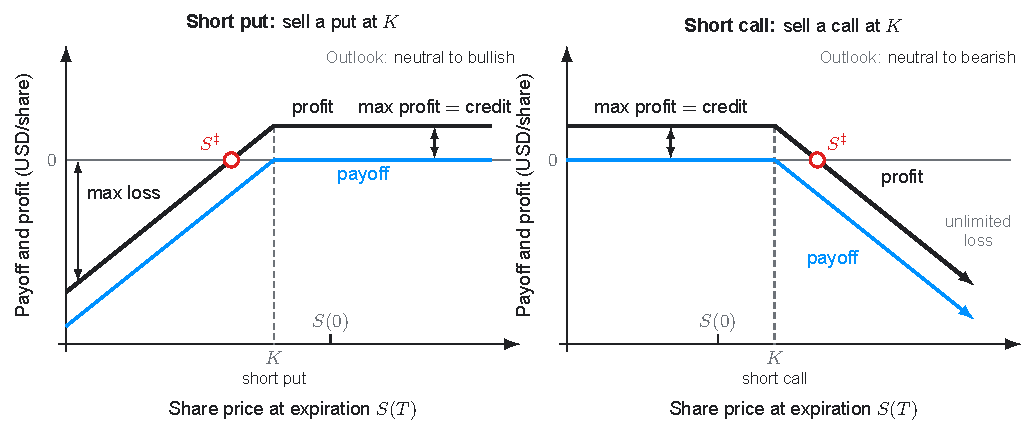
\includegraphics[width=\textwidth,height=0.58\textheight,keepaspectratio]{../figs/Fig-L10b-Short-Put-Call.pdf}
  \end{center}
  Each keeps the whole premium if it expires out of the money.
\end{frame}

\begin{frame}{Short Puts and Short Calls: Profit at Expiration}
  With premiums $\Pc_{p}$ (put) and $\Pc_{c}$ (call) at strike $K$, the profits
  at expiration, and the breakevens $S^{\ddagger}$, are:
  \begin{align*}
    \hat{P}_{\Cc}(S(T)) &= \Dc_{T,0}(g_{y})\cdot\Pc_{p}-(K-S(T))^{+} && \text{short put}\\
    \hat{P}_{\Cc}(S(T)) &= \Dc_{T,0}(g_{y})\cdot\Pc_{c}-(S(T)-K)^{+} && \text{short call}
  \end{align*}
  \begin{center}\small
    \begin{tabular}{lll}
      \toprule
      & Short put & Short call \\
      \midrule
      Maximum profit & $\Dc_{T,0}(g_{y})\cdot\Pc_{p}$ for $S(T)\geq K$ & $\Dc_{T,0}(g_{y})\cdot\Pc_{c}$ for $S(T)\leq K$ \\
      Breakeven & $S^{\ddagger}=K-\Dc_{T,0}(g_{y})\cdot\Pc_{p}$ & $S^{\ddagger}=K+\Dc_{T,0}(g_{y})\cdot\Pc_{c}$ \\
      Maximum loss & $K-\Dc_{T,0}(g_{y})\cdot\Pc_{p}$ at $S(T)=0$ & unlimited \\
      \bottomrule
    \end{tabular}
  \end{center}
  The short put's loss is bounded ($S(T)\geq0$); the short call's is not.
\end{frame}

\begin{frame}{Credit Spreads}
  A \hilite{credit spread} sells the contract closer to the share price and buys
  one farther away, same type and expiration (a
  \href{https://www.fidelity.com/learning-center/investment-products/options/options-strategy-guide/bull-put-spread}{\hilite{bull put}}
  or
  \href{https://www.fidelity.com/learning-center/investment-products/options/options-strategy-guide/bear-call-spread}{\hilite{bear call}}
  spread):
  \begin{center}
    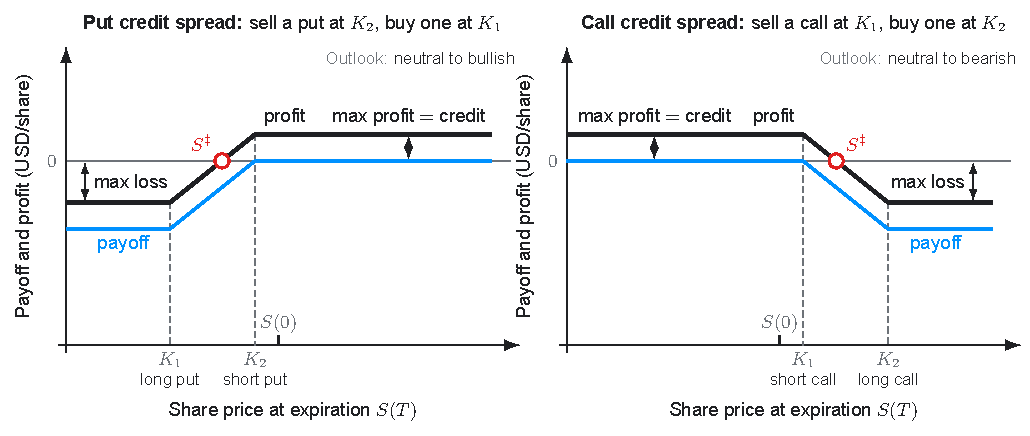
\includegraphics[width=\textwidth,height=0.55\textheight,keepaspectratio]{../figs/Fig-L10b-Credit-Spreads.pdf}
  \end{center}
  The short leg collects the credit; the long leg caps the loss.
\end{frame}

\begin{frame}{Put Credit Spread}
  A long put at $K_{1}$ and a short put at $K_{2}$: the credit grown to
  expiration, minus and plus the leg payoffs:
  \begin{equation*}
    \hat{P}_{\Cc}(S(T)) = \Dc_{T,0}(g_{y})\cdot(\Pc_{2}-\Pc_{1})-(K_{2}-S(T))^{+}+(K_{1}-S(T))^{+}
  \end{equation*}
  \begin{center}\small
    \begin{tabular}{ll}
      \toprule
      Maximum profit & $\Dc_{T,0}(g_{y})\cdot(\Pc_{2}-\Pc_{1})$ for $S(T)\geq K_{2}$ \\
      Breakeven & $S^{\ddagger}=K_{2}-\Dc_{T,0}(g_{y})\cdot(\Pc_{2}-\Pc_{1})$ \\
      Maximum loss & $(K_{2}-K_{1})-\Dc_{T,0}(g_{y})\cdot(\Pc_{2}-\Pc_{1})$ for $S(T)\leq K_{1}$ \\
      \bottomrule
    \end{tabular}
  \end{center}
  \slidenote{Example 3:}{\href{\repo/CHEME-5660-L10b-Example-Delta-VerticalSpread-Fall-2026.ipynb}{\dimmed{CHEME-5660-L10b-Example-Delta-VerticalSpread-Fall-2026.ipynb}}}
\end{frame}

\begin{frame}{Call Credit Spread}
  A short call at $K_{1}$ and a long call at $K_{2}$ give the profit at
  expiration:
  \begin{equation*}
    \hat{P}_{\Cc}(S(T)) = \Dc_{T,0}(g_{y})\cdot(\Pc_{1}-\Pc_{2})-(S(T)-K_{1})^{+}+(S(T)-K_{2})^{+}
  \end{equation*}
  \begin{center}\small
    \begin{tabular}{ll}
      \toprule
      Maximum profit & $\Dc_{T,0}(g_{y})\cdot(\Pc_{1}-\Pc_{2})$ for $S(T)\leq K_{1}$ \\
      Breakeven & $S^{\ddagger}=K_{1}+\Dc_{T,0}(g_{y})\cdot(\Pc_{1}-\Pc_{2})$ \\
      Maximum loss & $(K_{2}-K_{1})-\Dc_{T,0}(g_{y})\cdot(\Pc_{1}-\Pc_{2})$ for $S(T)\geq K_{2}$ \\
      \bottomrule
    \end{tabular}
  \end{center}
  Beyond the long strike, the long leg gains what the short leg loses, so the
  loss stops at the strike width minus the credit.
\end{frame}

\begin{frame}{Short Straddles and Strangles}
  A \href{https://www.fidelity.com/learning-center/investment-products/options/options-strategy-guide/short-straddle}{\hilite{straddle}}:
  a put and a call at one strike $K$. A
  \href{https://www.fidelity.com/learning-center/investment-products/options/options-strategy-guide/short-strangle}{\hilite{strangle}}: a
  put at $K_{1}$ below a call at $K_{2}$. Same expiration:
  \begin{center}
    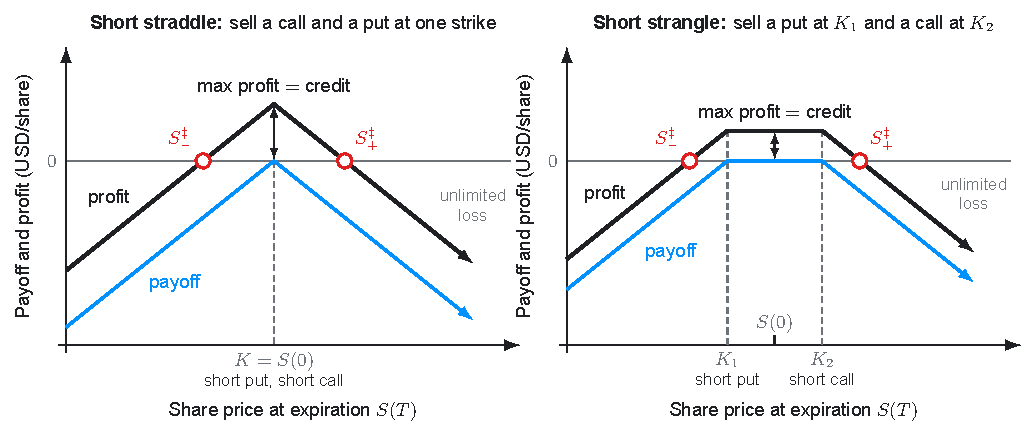
\includegraphics[width=\textwidth,height=0.55\textheight,keepaspectratio]{../figs/Fig-L10b-Straddle-Strangle.pdf}
  \end{center}
  Sold, each profits only between its breakevens:
  $\text{POP}=\mathbb{P}(S^{\ddagger}_{-}<S(T)<S^{\ddagger}_{+})$.
\end{frame}

\begin{frame}{Short Straddle}
  Selling a put and a call at the strike $K$ gives the profit at expiration:
  \begin{equation*}
    \hat{P}_{\Cc}(S(T)) = \Dc_{T,0}(g_{y})\cdot(\Pc_{p}+\Pc_{c})-(K-S(T))^{+}-(S(T)-K)^{+}
  \end{equation*}
  \begin{center}\small
    \begin{tabular}{ll}
      \toprule
      Maximum profit & $\Dc_{T,0}(g_{y})\cdot(\Pc_{p}+\Pc_{c})$ at $S(T)=K$ \\
      Lower breakeven & $S^{\ddagger}_{-}=K-\Dc_{T,0}(g_{y})\cdot(\Pc_{p}+\Pc_{c})$ \\
      Maximum loss below $S^{\ddagger}_{-}$ & $K-\Dc_{T,0}(g_{y})\cdot(\Pc_{p}+\Pc_{c})$ at $S(T)=0$ \\
      Upper breakeven & $S^{\ddagger}_{+}=K+\Dc_{T,0}(g_{y})\cdot(\Pc_{p}+\Pc_{c})$ \\
      Maximum loss above $S^{\ddagger}_{+}$ & unlimited \\
      \bottomrule
    \end{tabular}
  \end{center}
  The straddle collects more credit, but the strangle keeps its credit over a
  wider range of share prices.
\end{frame}

\begin{frame}{Short Strangle}
  Selling a put at $K_{1}$ and a call at $K_{2}$ gives the profit at expiration:
  \begin{equation*}
    \hat{P}_{\Cc}(S(T)) = \Dc_{T,0}(g_{y})\cdot(\Pc_{1}+\Pc_{2})-(K_{1}-S(T))^{+}-(S(T)-K_{2})^{+}
  \end{equation*}
  \begin{center}\small
    \begin{tabular}{ll}
      \toprule
      Maximum profit & $\Dc_{T,0}(g_{y})\cdot(\Pc_{1}+\Pc_{2})$ for $K_{1}\leq S(T)\leq K_{2}$ \\
      Lower breakeven & $S^{\ddagger}_{-}=K_{1}-\Dc_{T,0}(g_{y})\cdot(\Pc_{1}+\Pc_{2})$ \\
      Maximum loss below $S^{\ddagger}_{-}$ & $K_{1}-\Dc_{T,0}(g_{y})\cdot(\Pc_{1}+\Pc_{2})$ at $S(T)=0$ \\
      Upper breakeven & $S^{\ddagger}_{+}=K_{2}+\Dc_{T,0}(g_{y})\cdot(\Pc_{1}+\Pc_{2})$ \\
      Maximum loss above $S^{\ddagger}_{+}$ & unlimited \\
      \bottomrule
    \end{tabular}
  \end{center}
  \slidenote{Review on your own:}{\href{\repo/CHEME-5660-L10b-Example-Straddle-AMD-Earnings-Fall-2026.ipynb}{\dimmed{CHEME-5660-L10b-Example-Straddle-AMD-Earnings-Fall-2026.ipynb}}}
\end{frame}

\begin{frame}{Protected Strangles and Iron Condors}
  A \hilite{protected strangle}
  (\href{https://www.tastylive.com/concepts-strategies/jade-lizard}{\hilite{jade lizard}})
  adds a long call at $K_{3}$ to a short strangle; an
  \href{https://www.fidelity.com/learning-center/investment-products/options/options-strategy-guide/short-iron-condor-spread}{\hilite{iron condor}}
  also adds a long put:
  \begin{center}
    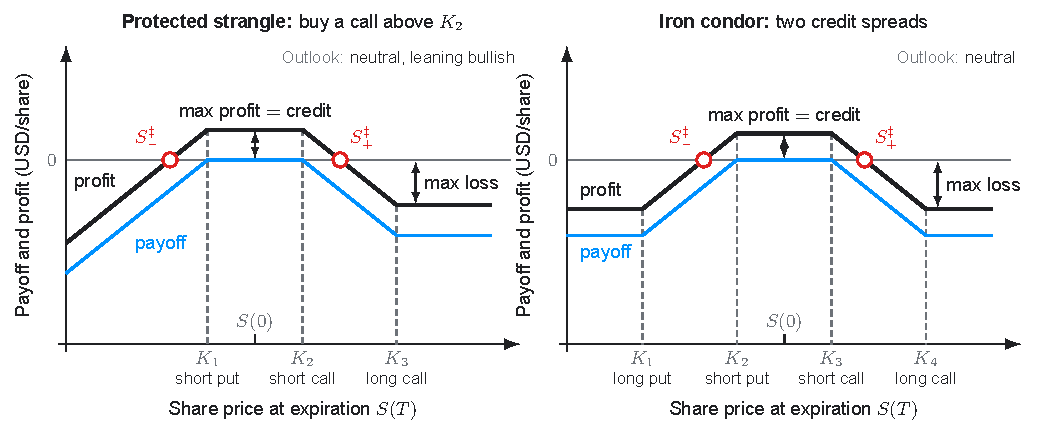
\includegraphics[width=\textwidth,height=0.58\textheight,keepaspectratio]{../figs/Fig-L10b-Protected-Condor.pdf}
  \end{center}
  Each long leg caps the loss on its side but lowers the credit.
\end{frame}

\begin{frame}{Protected Strangle}
  A short put at $K_{1}$, a short call at $K_{2}$, and a long call at $K_{3}$
  give the profit at expiration:
  \begin{align*}
    \hat{P}_{\Cc}(S(T)) &= \Dc_{T,0}(g_{y})\cdot(\Pc_{1}+\Pc_{2}-\Pc_{3}) && \text{protected strangle}\\
    &\qquad-(K_{1}-S(T))^{+}-(S(T)-K_{2})^{+}+(S(T)-K_{3})^{+}
  \end{align*}
  \begin{center}\footnotesize
    \begin{tabular}{ll}
      \toprule
      Maximum profit & $\Dc_{T,0}(g_{y})\cdot(\Pc_{1}+\Pc_{2}-\Pc_{3})$ for $K_{1}\leq S(T)\leq K_{2}$ \\
      Lower breakeven & $S^{\ddagger}_{-}=K_{1}-\Dc_{T,0}(g_{y})\cdot(\Pc_{1}+\Pc_{2}-\Pc_{3})$ \\
      Maximum loss below $S^{\ddagger}_{-}$ & $K_{1}-\Dc_{T,0}(g_{y})\cdot(\Pc_{1}+\Pc_{2}-\Pc_{3})$ at $S(T)=0$ \\
      Upper breakeven & $S^{\ddagger}_{+}=K_{2}+\Dc_{T,0}(g_{y})\cdot(\Pc_{1}+\Pc_{2}-\Pc_{3})$${}^{a}$ \\
      Maximum loss above $S^{\ddagger}_{+}$ & $(K_{3}-K_{2})-\Dc_{T,0}(g_{y})\cdot(\Pc_{1}+\Pc_{2}-\Pc_{3})$ for $S(T)\geq K_{3}$${}^{b}$ \\
      \bottomrule
    \end{tabular}
  \end{center}
  {\footnotesize ${}^{a}$If $\Dc_{T,0}(g_{y})\cdot(\Pc_{1}+\Pc_{2}-\Pc_{3})\leq K_{3}-K_{2}$; otherwise none. ${}^{b}$If $\Dc_{T,0}(g_{y})\cdot(\Pc_{1}+\Pc_{2}-\Pc_{3})<K_{3}-K_{2}$; otherwise none.\par}
  \vspace{0.3em}
  If the credit grown to expiration is at least $K_{3}-K_{2}$, the call side
  cannot lose.
\end{frame}

\begin{frame}{Iron Condor}
  A long put at $K_{1}$, a short put at $K_{2}$, a short call at $K_{3}$, and a
  long call at $K_{4}$ give the profit at expiration:
  \begin{align*}
    \hat{P}_{\Cc}(S(T)) &= \Dc_{T,0}(g_{y})\cdot(\Pc_{2}+\Pc_{3}-\Pc_{1}-\Pc_{4})\\
    &\qquad+(K_{1}-S(T))^{+}-(K_{2}-S(T))^{+}-(S(T)-K_{3})^{+}+(S(T)-K_{4})^{+}
  \end{align*}
  \begin{center}\footnotesize
    \begin{tabular}{ll}
      \toprule
      Maximum profit & $\Dc_{T,0}(g_{y})\cdot(\Pc_{2}+\Pc_{3}-\Pc_{1}-\Pc_{4})$ for $K_{2}\leq S(T)\leq K_{3}$ \\
      Lower breakeven & $S^{\ddagger}_{-}=K_{2}-\Dc_{T,0}(g_{y})\cdot(\Pc_{2}+\Pc_{3}-\Pc_{1}-\Pc_{4})$ \\
      Maximum loss below $S^{\ddagger}_{-}$ & $(K_{2}-K_{1})-\Dc_{T,0}(g_{y})\cdot(\Pc_{2}+\Pc_{3}-\Pc_{1}-\Pc_{4})$ for $S(T)\leq K_{1}$ \\
      Upper breakeven & $S^{\ddagger}_{+}=K_{3}+\Dc_{T,0}(g_{y})\cdot(\Pc_{2}+\Pc_{3}-\Pc_{1}-\Pc_{4})$ \\
      Maximum loss above $S^{\ddagger}_{+}$ & $(K_{4}-K_{3})-\Dc_{T,0}(g_{y})\cdot(\Pc_{2}+\Pc_{3}-\Pc_{1}-\Pc_{4})$ for $S(T)\geq K_{4}$ \\
      \bottomrule
    \end{tabular}
  \end{center}
  At any share price at expiration, at most one side can lose, so the maximum
  loss is the wider strike width minus the credit.
\end{frame}

\begin{frame}{Why Wait to Expiration?}
  Our diagrams are drawn at expiration. Closing a short leg early means buying it back: intrinsic plus extrinsic value
  $E_{V}(t)$. A short strangle (put $K_{1}=90$, call $K_{2}=110$, $S(0)=100$
  USD/share, 30 days, CRR tree, $\sigma=0.40$, $g_{y}=4\%$):
  \begin{center}
    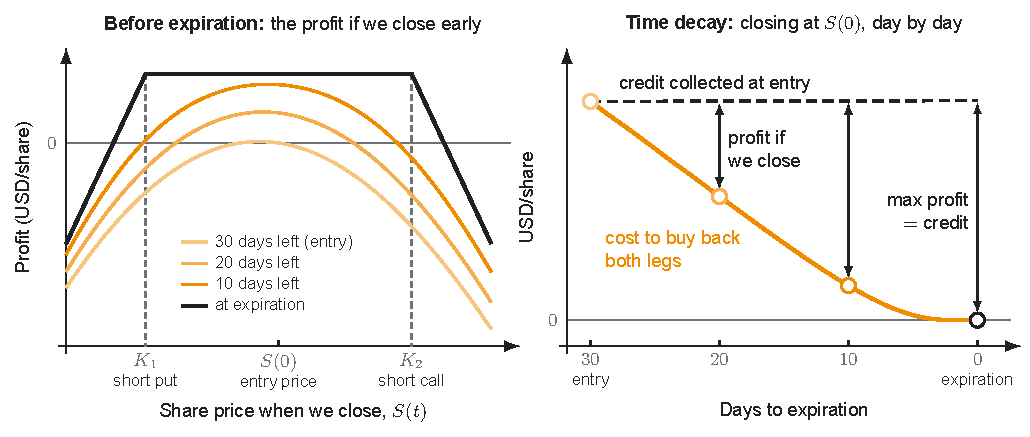
\includegraphics[width=\textwidth,height=0.55\textheight,keepaspectratio]{../figs/Fig-L10b-Strangle-Time-Decay.pdf}
  \end{center}
\end{frame}

\begin{frame}{Why Wait to Expiration? What Do We See?}
  \begin{itemize}\setlength{\itemsep}{0.6em}
    \item \hilite{Before expiration (left)}: the buyback price still includes
      extrinsic value, so earlier curves lie below the profit at expiration.
    \item \hilite{At the entry share price (right)}: both legs are out of the
      money, so closing at once costs exactly the credit and earns nothing.
    \item \hilite{Time decay}: as the extrinsic value decays, the profit if we
      close at $S(0)$ rises to the whole credit.
  \end{itemize}
  \vspace{0.4em}
  The diagrams show the most each contract can earn; an early exit earns less,
  by roughly the extrinsic value left in the legs.
\end{frame}

\begin{frame}{Summary}
  \vspace{0.3em}
  {\large\textbf{\ink{Key takeaways}}}
  \begin{itemize}\setlength{\itemsep}{0.4em}
    \item \hilite{POE, POP, and Delta}: both probabilities come from simulated
      share prices, and the size of Delta approximates the POE under $\Q$.
    \item \hilite{The NPV of a composite contract is a sum over its legs}: the POP
      is the probability that the profit at expiration is positive.
    \item \hilite{Common composite contracts can be bullish, bearish, or neutral}:
      the profit diagram gives the outlook, breakevens, and maximum loss; closing
      early earns less.
  \end{itemize}
\end{frame}

\end{document}
